\chapter{Erste Experimente mit dem EV3}
In diesem Abschnitt werden verschiedenes Experimente mit dem EV3 vorgestellt. Dazu zählen das kennenlernen der Sensoren so wie deren Zusammenspiel.
\section{Aufbau des Roboters} 
Anhand einer beiliegenden Anleitung wurde der Roboter zusammengebaut. Wie schon im Abschnitt \vref{lab:Antriebsart} beschrieben, erhält der Roboter zwei unabhängige Motoren für seine Räder sowie ein voll bewegliches Stützrad, realisiert durch eine Kugel.

Die Steuereinheit, im Folgenden auch \textit{Brick} genannt, ist oberhalb der Motoren so wie dem Stützrad angebracht. Die Motoren und Sensoren werden über Kabel mit dem Brick verbunden. 

Für die folgenden Experimente wurden Halterungen für die benötigten Sensoren bereitgehalten.   
   
\section{Aufbau und Test des Ultraschallsensors}
In diesem Abschnitt wird über den Test des Ultraschallsensors geschrieben. Das dargestellte Programm dient nur zu testzwecken und fand im späteren Verlauf des Projekts in dieser Version keine Verwendung mehr.
\paragraph{Aufbau und Programmierung des Roboters}
Der Roboter wurde mit Hilfe der beiliegenden Anleitung zusammengebaut. Er besitzt zwei Motoren, die jeweils eines der Räder antreiben. Damit das Heck nicht auf dem Untergrund aufsetzt, wurde eine freilaufende Kugel installiert. 
Als Sensor wurde bei diesem Aufbau der Ultraschallsensor verwendet. Er dient zu Hinderniserkennung und hat einen Arbeitsbereich von 3-250cm.

\paragraph{Ziel}
Der Roboter soll nach dem einprogrammierten Muster in einer ihm unbekannten Umgebung selbstständig Hindernissen ausweichen. Der Ultraschallsensor soll die Hindernisse erkennen. Dieser Versuch soll helfen, die Grenzen des Sensors kennenzulernen. Des weiteren dient dieser Versuchsaufbau dazu weitere Eigenheiten des Roboters kennenzulernen. Auch soll der Aufbau als Grundgerüst für weitere Sensoren und Versuche dienen.  

Der Roboter wird mit einer von Lego Entworfenen Programmierumgebung programmiert. Diese Umgebung ist eine grafische Programmierung des Bricks. Diese Programmierumgebung soll im laufe des Projekts benutzt und getestet werden.

\paragraph{Testprogramm des Ultraschallsensors}
\begin{figure}[htb]
\centering
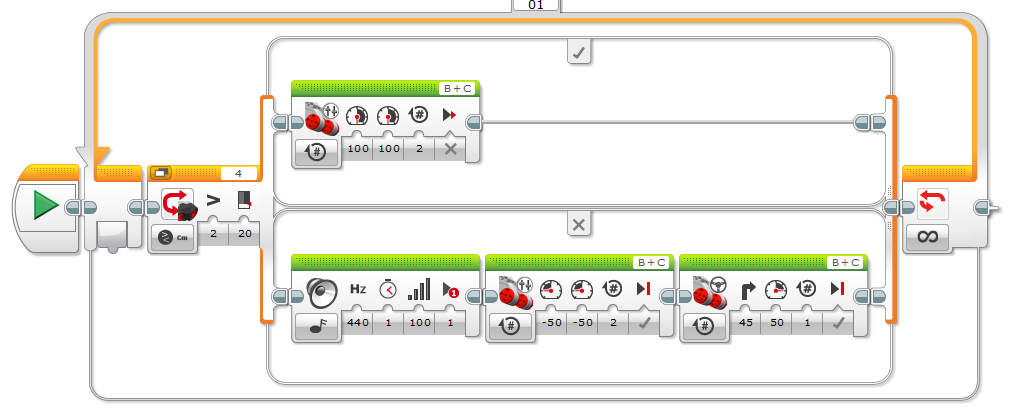
\includegraphics[width= 15cm]{Prog_Ultraschallsensor}
\caption{Lego-Programm zum Test und Kennenlernen des Ultraschallsensor}
\label{fig:ultraschallsensorprog}
\end{figure}
Im der Abbildung \vref{fig:ultraschallsensorprog} wird das, mit der Lego- Programmierumgebung erstellte, Programm dargestellt.\\
Das Programm besteht aus zwei ineinander geschachtelte Schleifen. Die äußere Schleife besitzt keine Abbruchbedingung. Die innere der beiden Schleifen überwacht den Ultraschallsensor und entscheidet je nach Ergebnis des Sensors, was der Roboter machen soll.\\
Trifft der Vergleich \textbf{Vergleich erläutern} zu so fährt der Roboter mit Höchstgeschwindigkeit nach vorne, solange bis sich jedes der Räder genau zweimal gedreht hat. Danach wird auf Grund der Endlosschleife wieder der Ultraschallsensor abgefragt. Diesen Zweig erkennt man an dem Haken über den Anweisungen.

Trifft der Vergleich nicht zu, wird zuerst ein Ton über den integrierten Lautsprecher ausgegeben. Dieser Ton ist ein 440Hz Ton und wird mit voller Lautstärke eine Sekunde lang ausgegeben. Anschliesend fährt der Roboter mit halber Kraft zwei Radumdrehung zurück. Ist dies erledigt, soll sich der Roboter um 45 Grad drehen. Aufgrund der Endlosschleife wird wieder von Vorne begonnen und der Ultraschallsensor wird abgefragt. Dieser Zweig ist in der Darstellung \vref{fig:ultraschallsensorprog} an dem darüber stehenden x zuerkennen.
 
\paragraph{Beobachtungen} Bei den Versuchen wurde festgestellt, dass die Hindernisse eine gewisse Breite und auch Höhe haben müssen, damit der Sensor sie wahrnimmt.
Damit die Sensoren zeitlich relativ gute Ergebnisse liefern, dürfen die Schleifen der Sensoren nicht zu viele andere Programmbausteine besitzen. Dies kann dazuführen, dass der Sensor seine Abfrage zu spät ausführt und dadurch schon auf ein Hindernis gestoßen ist.

Des weiteren wurde bei den Tests festgestellt, dass der Roboter im jetzigen Aufbau auf diversen Oberflächen, wie Teppich, Fliesen oder Parkett, verschieden große Kurvenradien fährt. Dieses Verhalten liegt an den unterschiedlichen Reibungswerten des jeweiligen Untergrunds.

Innerhalb der Programmierumgebung wurde festgestellt, dass die Übersichtlichkeit mit Zunahme der Komplexität abnimmt. Zum Testen der Sensoren und Aktoren des Roboters ist die Programmierumgebung geeignet.

Als positiv zu werten ist die Darstellung der Sensoren. Bei bestehender Verbindung mit dem EV3 kann der Anwender die Sensorwerte direkt in der Programmierumgebung nachvollziehen.

\paragraph{Auswertung}
Das Programm zum Ausweichen von Gegenständen ist in Abbildung \vref{fig:ultraschallsensorprog} dargestellt und näher erläutert. Die Programmierumgebung ist zum einarbeiten und kennenlernen der Sensoren geeignet. Jedoch wird das Programm je komplexer es wird auch unübersichtlicher. Die Umgebung zeigt bei bestehender Verbindung zwischen PC und Brick die Echtzeitdaten der Motoren und Sensoren an. Dies unterstützt beim kennenlernen der Sensoren und hilft bei Problemen. So wurde festgestellt, dass der Ultraschallsensor Gegenstände, die eine gewisse Breite(Breite unter 2-5 cm) nicht erfüllen, nur fehlerhaft oder gar nicht erkannt werden.  

\section{Test des mitgelieferten Farbsensors}
\paragraph{Aufbau}
Der Lego eigene Farbsensor wird zuerst nur über ein Kabel mit dem \underline{Brick} verbunden. 

Getestet wurde der Sensor wieder mit der Software von Lego. Dort wurde für die Erkennung von Farben die entsprechenden Parameter eingestellt, damit der Sensor verschiedene Farben erkennen kann. Dies sind acht verschiedene Farben, die von farblos über Gelb und Grün bis hin zu Rot und Schwarz reichen.

Im ersten Test zum kennenlernen wurde auf ein gleichzeitiger Einsatz von Ultraschallsensor und Farbsensor verzichtet.

Im zweiten Test wird der Sensor fest am Roboter verbaut und auf den Boden gerichtet. Aufgrund des vorigen Tests wird der Sensor nicht zu weit über dem Boden montiert. Mit entsprechender Programmierung soll der Roboter solange fahren, bis sich auf dem Boden eine Markierung mit einer anderen Farbe befindet. Wird dies festgestellt, soll der Roboter anhalten.  
\paragraph{Testprogramm des Lego-Farbsensor}
\begin{figure}[htb]
\centering
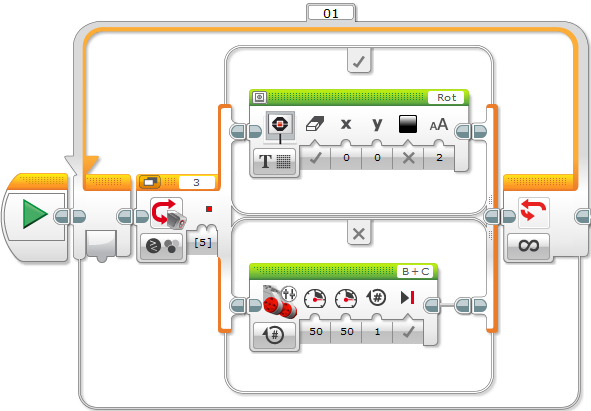
\includegraphics[width= 14cm]{Prog_LichtsensorLego_v1}
\caption{Lego-Programm zum Test und Kennenlernen des Farbsensors von Lego}
\label{fig:farbsensorprog}
\end{figure}
Das unter Abblidung\vref{fig:farbsensorprog} dargestellte Programm, ist ein Beispielprogramm für den Lego eigenen Farbsensor. 
Mit Hilfe dieses Programms wurde festgestellt, dass der Sensor manche Farben fehlerhaft erkennt. Dies ist zurückzuführen auf seine niedrige Farbauflösung. Diese Detektiert lediglich acht verschiedene Farben.
\paragraph{Ziel}
Ziel dieser Tests ist es den Sensor kennenzulernen. Hierzu zählen die notwendigen Abstände des Sensors, so wie die möglichen Farben die der Sensor erkennen könnte.
Ebenfalls soll mit dem Test festgestellt werden, ob der Sensor für das Projekt genutzt werden kann. Dazu wird ein Programm geschrieben, in dem sich der Roboter bewegt und sobald er eine andere, noch nicht festgelegte, Farbe auf dem Boden erkennt, anhält. 
- Sensor kennenlernen\\
- Sensor einsetzen können\\
- Feststellung ob der Sensor für das Projekt geeignet ist

\paragraph{Beobachtungen}
Während dem ersten Teil des Tests, als der Sensor noch nicht fest am Roboter gefestigt war, wurde festgestellt, dass der Sensor einen gewissen Bereich hat in dem es zu Fehlmessungen kommen kann. Zusätzlich dazu war festzustellen, dass der Sensor bei Mischfarben falsche Farbwerte liefert. Er zeigte beispielsweise bei einer Mischung aus grüner und brauner Farbe, dass er die Farbe schwarz erkannt hätte.
\paragraph{Auswertung}
-Bedingt einsetzbar für das Projekt.\\
Grund :$\Rightarrow$ Farben müssen eindeutig sein und dürfen keine Mischfarben sein.



